\documentclass{sigchi}

% Use this section to set the ACM copyright statement (e.g. for
% preprints).  Consult the conference website for the camera-ready
% copyright statement.

% Copyright
%\CopyrightYear{2020}
%\setcopyright{acmcopyright}
%\setcopyright{acmlicensed}
%\setcopyright{rightsretained}
%\setcopyright{usgov}
%\setcopyright{usgovmixed}
%\setcopyright{cagov}
%\setcopyright{cagovmixed}
% DOI
%\doi{https://doi.org/10.1145/3313831.XXXXXXX}
% ISBN
%\isbn{978-1-4503-6708-0/20/04}
%Conference
%\conferenceinfo{CHI'20,}{April  25--30, 2020, Honolulu, HI, USA}
%Price
%\acmPrice{\$15.00}

% Use this command to override the default ACM copyright statement
% (e.g. for preprints).  Consult the conference website for the
% camera-ready copyright statement.

\toappear{\scriptsize
 Copyright (c) 2020 for this paper by its authors. Use permitted under Creative Commons License Attribution 4.0 International (CC BY 4.0). \\
 \emph{IntRS '20 - Joint Workshop on Interfaces and Human Decision Making for Recommender Systems},  September 26, 2020, Virtual Event}

\clubpenalty=10000
\widowpenalty = 10000

%% HOW TO OVERRIDE THE DEFAULT COPYRIGHT STRIP --
%% Please note you need to make sure the copy for your specific
%% license is used here!
% \toappear{
% Permission to make digital or hard copies of all or part of this work
% for personal or classroom use is granted without fee provided that
% copies are not made or distributed for profit or commercial advantage
% and that copies bear this notice and the full citation on the first
% page. Copyrights for components of this work owned by others than ACM
% must be honored. Abstracting with credit is permitted. To copy
% otherwise, or republish, to post on servers or to redistribute to
% lists, requires prior specific permission and/or a fee. Request
% permissions from \href{mailto:Permissions@acm.org}{Permissions@acm.org}. \\
% \emph{CHI '16},  May 07--12, 2016, San Jose, CA, USA \\
% ACM xxx-x-xxxx-xxxx-x/xx/xx\ldots \$15.00 \\
% DOI: \url{http://dx.doi.org/xx.xxxx/xxxxxxx.xxxxxxx}
% }

% Arabic page numbers for submission.  Remove this line to eliminate
% page numbers for the camera ready copy
% \pagenumbering{arabic}

% Load basic packages
\PassOptionsToPackage{usenames,dvipsnames}{xcolor}
\PassOptionsToPackage{colorlinks,linktoc=all}{hyperref}
\usepackage{balance}       % to better equalize the last page
\usepackage{graphics}      % for EPS, load graphicx instead 
\usepackage[T1]{fontenc}   % for umlauts and other diaeresis
\usepackage{txfonts}
\usepackage{mathptmx}
\usepackage{color}
\usepackage{booktabs}
\usepackage{textcomp}
\usepackage{cuted}
\usepackage{capt-of}
\usepackage[pdflang={en-US},pdftex]{hyperref}

% Some optional stuff you might like/need.
\usepackage{microtype}        % Improved Tracking and Kerning
% \usepackage[all]{hypcap}    % Fixes bug in hyperref caption linking
\usepackage{ccicons}          % Cite your images correctly!
% \usepackage[utf8]{inputenc} % for a UTF8 editor only

% If you want to use todo notes, marginpars etc. during creation of
% your draft document, you have to enable the "chi_draft" option for
% the document class. To do this, change the very first line to:
% "\documentclass[chi_draft]{sigchi}". You can then place todo notes
% by using the "\todo{...}"  command. Make sure to disable the draft
% option again before submitting your final document.
\usepackage{todonotes}

% Paper metadata (use plain text, for PDF inclusion and later
% re-using, if desired).  Use \emtpyauthor when submitting for review
% so you remain anonymous.
\def\plaintitle{Recommending Interesting Writing using a Controllable, Explanation-Aware Visual Interface}
\def\plainauthor{Rohan Bansal, Jordan Olmstead, Uri Bram, Robert Cottrell, Gabriel Reder, Jaan Altosaar}
\def\emptyauthor{}
\def\plainkeywords{content-based recommendation, open source, visual interface}
\def\plaingeneralterms{Documentation, Standardization}

% llt: Define a global style for URLs, rather that the default one
\makeatletter
\def\url@leostyle{%
  \@ifundefined{selectfont}{
    \def\UrlFont{\sf}
  }{
    \def\UrlFont{\small\bf\ttfamily}
  }}
\makeatother
\urlstyle{leo}

% To make various LaTeX processors do the right thing with page size.
\def\pprw{8.5in}
\def\pprh{11in}
\special{papersize=\pprw,\pprh}
\setlength{\paperwidth}{\pprw}
\setlength{\paperheight}{\pprh}
\setlength{\pdfpagewidth}{\pprw}
\setlength{\pdfpageheight}{\pprh}

% Make sure hyperref comes last of your loaded packages, to give it a
% fighting chance of not being over-written, since its job is to
% redefine many LaTeX commands.
\definecolor{linkColor}{RGB}{6,125,233}
\hypersetup{%
  pdftitle={\plaintitle},
% Use \plainauthor for final version.
  pdfauthor={\plainauthor},
  pdfkeywords={\plainkeywords},
  pdfdisplaydoctitle=true, % For Accessibility
  bookmarksnumbered,
  pdfstartview={FitH},
  colorlinks,
  citecolor=black,
  filecolor=black,
  linkcolor=black,
  urlcolor=linkColor,
  breaklinks=true,
  hypertexnames=false
}

% create a shortcut to typeset table headings
% \newcommand\tabhead[1]{\small\textbf{#1}}

% !TEX root = ../recommending-interesting-writing.tex

% FONTS
%\usepackage[T1]{fontenc}

% Replace default Latin Modern typewriter with its proportional counterpart
% http://www.tug.dk/FontCatalogue/lmoderntypewriterprop/
%\renewcommand*\ttdefault{lmvtt}

%%% OPTION 3 - MTPRO 2 Math + Termes Times + ParaType Sans
\let\myBbbk\Bbbk
\let\Bbbk\relax
\let\bibsep\relax
\let\openbox\relax
\let\proof\relax
\let\endproof\relax
%\usepackage{tgtermes}
\usepackage{minted}
\usepackage{amsmath}
% \usepackage[subscriptcorrection,
%             amssymbols,
%             mtpbb,
%             mtpcal,
%             nofontinfo  % suppresses all warnings
%            ]{mtpro2}
% \usepackage{scalefnt,letltxmacro}
% \LetLtxMacro{\oldtextsc}{\textsc}
% \renewcommand{\textsc}[1]{\oldtextsc{\scalefont{1.10}#1}}
% \usepackage[scaled=0.92]{PTSans}

% ICONS
\usepackage{fontawesome}

% CODE

% COLOR
\usepackage[usenames,dvipsnames]{xcolor}
\definecolor{shadecolor}{gray}{0.9}

% SPACING and TEXT
%\usepackage[final,expansion=alltext]{microtype}
%\usepackage[english]{babel}
\usepackage[parfill]{parskip}
\usepackage{afterpage}
\usepackage{framed}
\usepackage{nicefrac}

% EDITING
% line numbering in left margin
\usepackage{lineno}
\renewcommand\linenumberfont{\normalfont
                             \footnotesize
                             \sffamily
                             \color{SkyBlue}}
% ragged paragraphs in right margin
\usepackage{ragged2e}
\DeclareRobustCommand{\sidenote}[1]{\marginpar{
                                    \RaggedRight
                                    \textcolor{Plum}{\textsf{#1}}}}

% Define a paragraph header function
\DeclareRobustCommand{\parhead}[1]{\textbf{#1}~}

% paragraph helper
\DeclareRobustCommand{\PP}{\textcolor{Plum}{\P}~}
\DeclareRobustCommand{\pp}{\textcolor{Plum}{\P}~}

% COUNTERS
\renewcommand{\labelenumi}{\color{black!67}{\arabic{enumi}.}}
\renewcommand{\labelenumii}{{\color{black!67}(\alph{enumii})}}
\renewcommand{\labelitemi}{{\color{black!67}\textbullet}}

% FIGURES
\usepackage{graphicx}
\usepackage[labelfont=bf]{caption}
\usepackage[format=hang]{subcaption}

% TABLES
\usepackage{booktabs}
%\usepackage{dblfloatfix}  % for placing table at bottom of page

% TABLE ALIGNMENT
\usepackage{etoolbox,siunitx}
\robustify\bfseries
\sisetup{detect-weight=true, detect-shape=true, detect-mode=true,
table-format=5.1,
table-number-alignment=center,
separate-uncertainty=true,
input-ignore={,},input-decimal-markers={.}}

% BABEL
% \usepackage{polyglossia}

% BIBLIOGRAPHY
\usepackage[backend=biber, style=numeric-comp]{biblatex}
%\usepackage{natbib}

% ALGORITHMS
\usepackage[algoruled]{algorithm2e}
\usepackage{listings}
\usepackage{fancyvrb}
\fvset{fontsize=\normalsize}

% THEOREMS
\usepackage{amsthm}
\newtheorem{theorem}{Theorem}
% \newtheorem{proposition}[proposition]{Proposition}
\newtheorem{prop}{Proposition}


% TODO
%\usepackage{todo}

% HYPERREF
%\usepackage[colorlinks,linktoc=all]{hyperref}
\usepackage[all]{hypcap}
\hypersetup{citecolor=Violet}
\hypersetup{linkcolor=black}
\hypersetup{urlcolor=MidnightBlue}

% CLEVEREF must come after HYPERREF
\usepackage[capitalize]{cleveref}

% ACRONYMS
\usepackage[acronym,smallcaps,nowarn]{glossaries}
% \makeglossaries

% COLOR DEFINITIONS
\newcommand{\red}[1]{\textcolor{BrickRed}{#1}}
\newcommand{\orange}[1]{\textcolor{BurntOrange}{#1}}
\newcommand{\green}[1]{\textcolor{OliveGreen}{#1}}
\newcommand{\blue}[1]{\textcolor{MidnightBlue}{#1}}
\newcommand{\gray}[1]{\textcolor{black!60}{#1}}

% LISTINGS DEFINTIONS
\usepackage{listings}
\lstdefinestyle{alp_style}{
    commentstyle=\color{OliveGreen},
    numberstyle=\tiny\color{black!60},
    stringstyle=\color{BrickRed},
    basicstyle=\ttfamily\scriptsize,
    breakatwhitespace=false,
    breaklines=true,
    captionpos=b,
    keepspaces=true,
    numbers=none,
    numbersep=5pt,
    showspaces=false,
    showstringspaces=false,
    showtabs=false,
    tabsize=2
}
\lstset{style=alp_style}

% !TEX root = ../set_recommendation.tex

\DeclareRobustCommand{\mb}[1]{\ensuremath{\boldsymbol{\mathbf{#1}}}}
%\DeclareRobustCommand{\mb}[1]{\mathbold{#1}}

\DeclareRobustCommand{\KL}[2]{\ensuremath{\textrm{KL}\left(#1\;\|\;#2\right)}}

\DeclareMathOperator*{\argmax}{arg\,max}
\DeclareMathOperator*{\argmin}{arg\,min}

\newcommand{\yum}{y_{um}}
\newcommand{\xum}{x_{um}}
\newcommand{\xuk}{x_{uk}}
\newcommand{\yuk}{y_{uk}}
\renewcommand{\mid}{~\vert~}
\newcommand{\prm}{\:;\:}

\newcommand{\mbw}{\mb{w}}
\newcommand{\mbW}{\mb{W}}

\newcommand{\mbx}{\mb{x}}
\newcommand{\mbX}{\mb{X}}

\newcommand{\mby}{\mb{y}}
\newcommand{\mbY}{\mb{Y}}

\newcommand{\mbz}{\mb{z}}
\newcommand{\mbZ}{\mb{Z}}

\newcommand{\mbI}{\mb{I}}
\newcommand{\mbone}{\mb{1}}

\newcommand{\mbL}{\mb{L}}

\newcommand{\mbtheta}{\mb{\theta}}
\newcommand{\mbTheta}{\mb{\Theta}}
\newcommand{\mbomega}{\mb{\omega}}
\newcommand{\mbOmega}{\mb{\Omega}}
\newcommand{\mbsigma}{\mb{\sigma}}
\newcommand{\mbSigma}{\mb{\Sigma}}
\newcommand{\mbphi}{\mb{\phi}}
\newcommand{\mbPhi}{\mb{\Phi}}

\newcommand{\mbalpha}{\mb{\alpha}}
\newcommand{\mbbeta}{\mb{\beta}}
\newcommand{\mbgamma}{\mb{\gamma}}
\newcommand{\mbeta}{\mb{\eta}}
\newcommand{\mbmu}{\mb{\mu}}
\newcommand{\mbrho}{\mb{\rho}}
\newcommand{\mblambda}{\mb{\lambda}}
\newcommand{\mbzeta}{\mb{\zeta}}

\newcommand\dif{\mathop{}\!\mathrm{d}}
\newcommand{\diag}{\textrm{diag}}
\newcommand{\supp}{\textrm{supp}}

\newcommand{\E}{\mathbb{E}}
\newcommand{\V}{\mathbb{V}}
\newcommand{\bbH}{\mathbb{H}}

\newcommand{\bbN}{\mathbb{N}}
\newcommand{\bbZ}{\mathbb{Z}}
\newcommand{\bbR}{\mathbb{R}}
\newcommand{\bbS}{\mathbb{S}}

\newcommand{\cL}{\mathcal{L}}
\newcommand{\cS}{\mathcal{S}}
\newcommand{\cD}{\mathcal{D}}

\newcommand{\cN}{\mathcal{N}}
\newcommand{\cT}{\mathcal{T}}

\newcommand{\mult}{\textrm{Mult}}
\newcommand{\dirichlet}{\textrm{Dirichlet}}
\newcommand{\Gam}{\textrm{Gamma}}
\newcommand{\Pois}{\textrm{Poisson}}
% !TEX root = recommending-interesting-writing.tex

\newacronym{ELBO}{elbo}{evidence lower bound}
\newacronym{GMM}{gmm}{Gaussian mixture model}
\newacronym{KL}{kl}{Kullback-Leibler}
\newacronym{LDA}{lda}{latent Dirichlet allocation}
\newacronym{SVI}{svi}{stochastic variational inference}
\newacronym{DEF}{def}{deep exponential family}
\newacronym{rfs}{rfs}{\textsc{rankfromsets}}
\newacronym{ctpf}{ctpf}{collaborative topic Poisson factorization}
\bibliography{bib} 
% End of preamble. Here it comes the document.
\begin{document}

\title{\plaintitle}

\numberofauthors{6}
\author{%
  \alignauthor{Rohan Bansal\\
    \affaddr{The Browser}\\
    \email{rohan@thebrowser.com}}\\
  \alignauthor{Jordan Olmstead\\
    \affaddr{The Browser}\\
    \email{jordan@thebrowser.com}}\\
  \alignauthor{Uri Bram\\
    \affaddr{The Browser}\\
    \email{uri@thebrowser.com}}\\
  \alignauthor{Robert Cottrell\\
    \affaddr{The Browser}\\
    \email{robert@thebrowser.com}}\\
  \alignauthor{Gabriel Reder\\
    \affaddr{Stanford University}\\
    \email{gkreder@stanford.edu}}\\
  \alignauthor{Jaan Altosaar\\
    \affaddr{Princeton University}\\
    \email{altosaar@princeton.edu}}\\
}

\maketitle
\begin{strip}\centering

\includegraphics[width=\textwidth]{fig/pipeline.pdf}
\captionof{figure}{End-to-end pipeline for recommending writing to editors at The Browser with a controllable, explanation-aware visual interface. The \acrlong{rfs} recommendation model~\parencite{altosaar2020rankfromsets:} is trained on data consisting of positive examples from the editors' history of curated articles, and negative examples from news sources. After training and offline evaluation of the recommendation model, \acrlong{rfs} is deployed as a microservice on Amazon Web Services Lambda, with the visual interface hosted on Github Pages. Editors can control the recommender system using the visual interface, which can aid in their decision-making. The editors' interrogation of the recommendation model informs further data collection and training.
\label{fig:pipeline}}
\end{strip}

% !TEX root = recommending-interesting-writing.tex
\begin{abstract}
  We build a visual interface for recommending articles to editors at The Browser, a curation service for interesting writing. From a large list of candidates, editors decide which articles are selected and shared with subscribers. To aid the editors in this decision-making task, we build a visual interface for a recommendation model, \gls{rfs}~\citep{altosaar2020rankfromsets:}, that classifies articles based on their words. Control of the recommendation model is built into the visual interface. For example, an editor can use a topic slider to receive a new list of recommendations according to topical words in articles. These topic sliders might be used to increase or decrease the ranking of articles with words related to crime, business, or technology. The visual interface is also designed to be explanation-aware: words that contribute positively or negatively to an article's ranking are displayed. For the backend of the visual interface, \gls{rfs} is trained on historical data. In an offline empirical study, we find that \gls{rfs} outperforms \acrshort{bert}~\citep{devlin2019bert:}, a competitive classification model, in terms of recall. Further, we measure \gls{rfs} to be 10 times faster to train and to return predictions 2000 times faster than \acrshort{bert}. This speed is a beneficial property for the visual interface, and we demonstrate that \gls{rfs} can be deployed on the free tier of AWS Lambda using a short python script and numpy dependency. For reproducibility, transparency, and trust of the visual interface, we open source and release a public demonstration,\footnote{\url{https://the-browser.github.io/recommending-interesting-writing/}\label{url:demo}} data collection, training and deployment scripts, and model parameters.\footnote{\url{https://github.com/the-browser/recommending-interesting-writing}}
\end{abstract}


% ACM Classfication

\begin{CCSXML}
<ccs2012>
   <concept>
       <concept_id>10010405.10010497.10010498</concept_id>
       <concept_desc>Applied computing~Document searching</concept_desc>
       <concept_significance>500</concept_significance>
       </concept>
   <concept>
       <concept_id>10010147.10010257.10010282.10010292</concept_id>
       <concept_desc>Computing methodologies~Learning from implicit feedback</concept_desc>
       <concept_significance>500</concept_significance>
       </concept>
 </ccs2012>
\end{CCSXML}

\ccsdesc[500]{Applied computing~Document searching}
\ccsdesc[500]{Computing methodologies~Learning from implicit feedback}

% Author Keywords
\keywords{content-based recommendation, open source, visual interface}

% Print the classficiation codes
\printccsdesc
Please use the 2012 Classifiers and see this link to embed them in the text: \url{https://dl.acm.org/ccs/ccs_flat.cfm}


\maketitle
% !TEX root = recommending-interesting-writing.tex
\section{Introduction}
\label{sec:introduction}
Creative nonfiction, longform journalism, and blog posts are examples of the types of articles curated by The Browser's team of editors. The editors read a large number of articles from various publications to select content to recommend to subscribers.

In building a recommender system to help editors sift through many documents, it is motivating to highlight the trade-off in user privacy intrinsic to recommender systems. A machine learning model must exploit information about a user. However, the incentive structures of operating a recommender system within a business can influence decisions around privacy and transparency~\citep{diakopoulos2020oxford}. For example, business models that rely on online advertising may engender recommender systems that upweight attention-grabbing content and hence time spent looking at ads. Such content might maximize a user's time spent with a service over time at the expense of long-term user experience or consent. In comparison, privacy-preserving and open source tools such as the Signal encrypted messaging service\footnote{\url{https://signal.org/}} may provide improved user experience in terms of privacy-preserving, transparent, and explainable algorithms and visual interfaces~\citep{cohn-gordon2017a-formal}. But the incentive structures for releasing recommender systems and visual interfaces that exploit private information about users are poor. There are few examples of end-to-end, open source, free-to-deploy pipelines for recommending content to users using a visual interface. This motivates building and deploying a recommendation model and corresponding explanation-aware visual interface to give users control, and inform them about how data is being used to make recommendations.

We build an end-to-end recommender system visual interface to address two aims: (1) to aid editors at The Browser in their decision-making task, and give them control through an explanation-aware interface, and (2) to release a lightweight, performant, open-source visual interface framework for explanation-aware recommender systems for document recommendation. In an offline evaluation, we show that the recommendation model we use for the visual interface outperforms \acrshort{bert}, a competitive document classification model. In a qualitative study, the control and explanations provided by the visual interface help editors in their decision-making and help find bugs in the recommendation model.

% !TEX root = ../recommending-interesting-writing.tex
\begin{figure}[!tb]
  \centering
  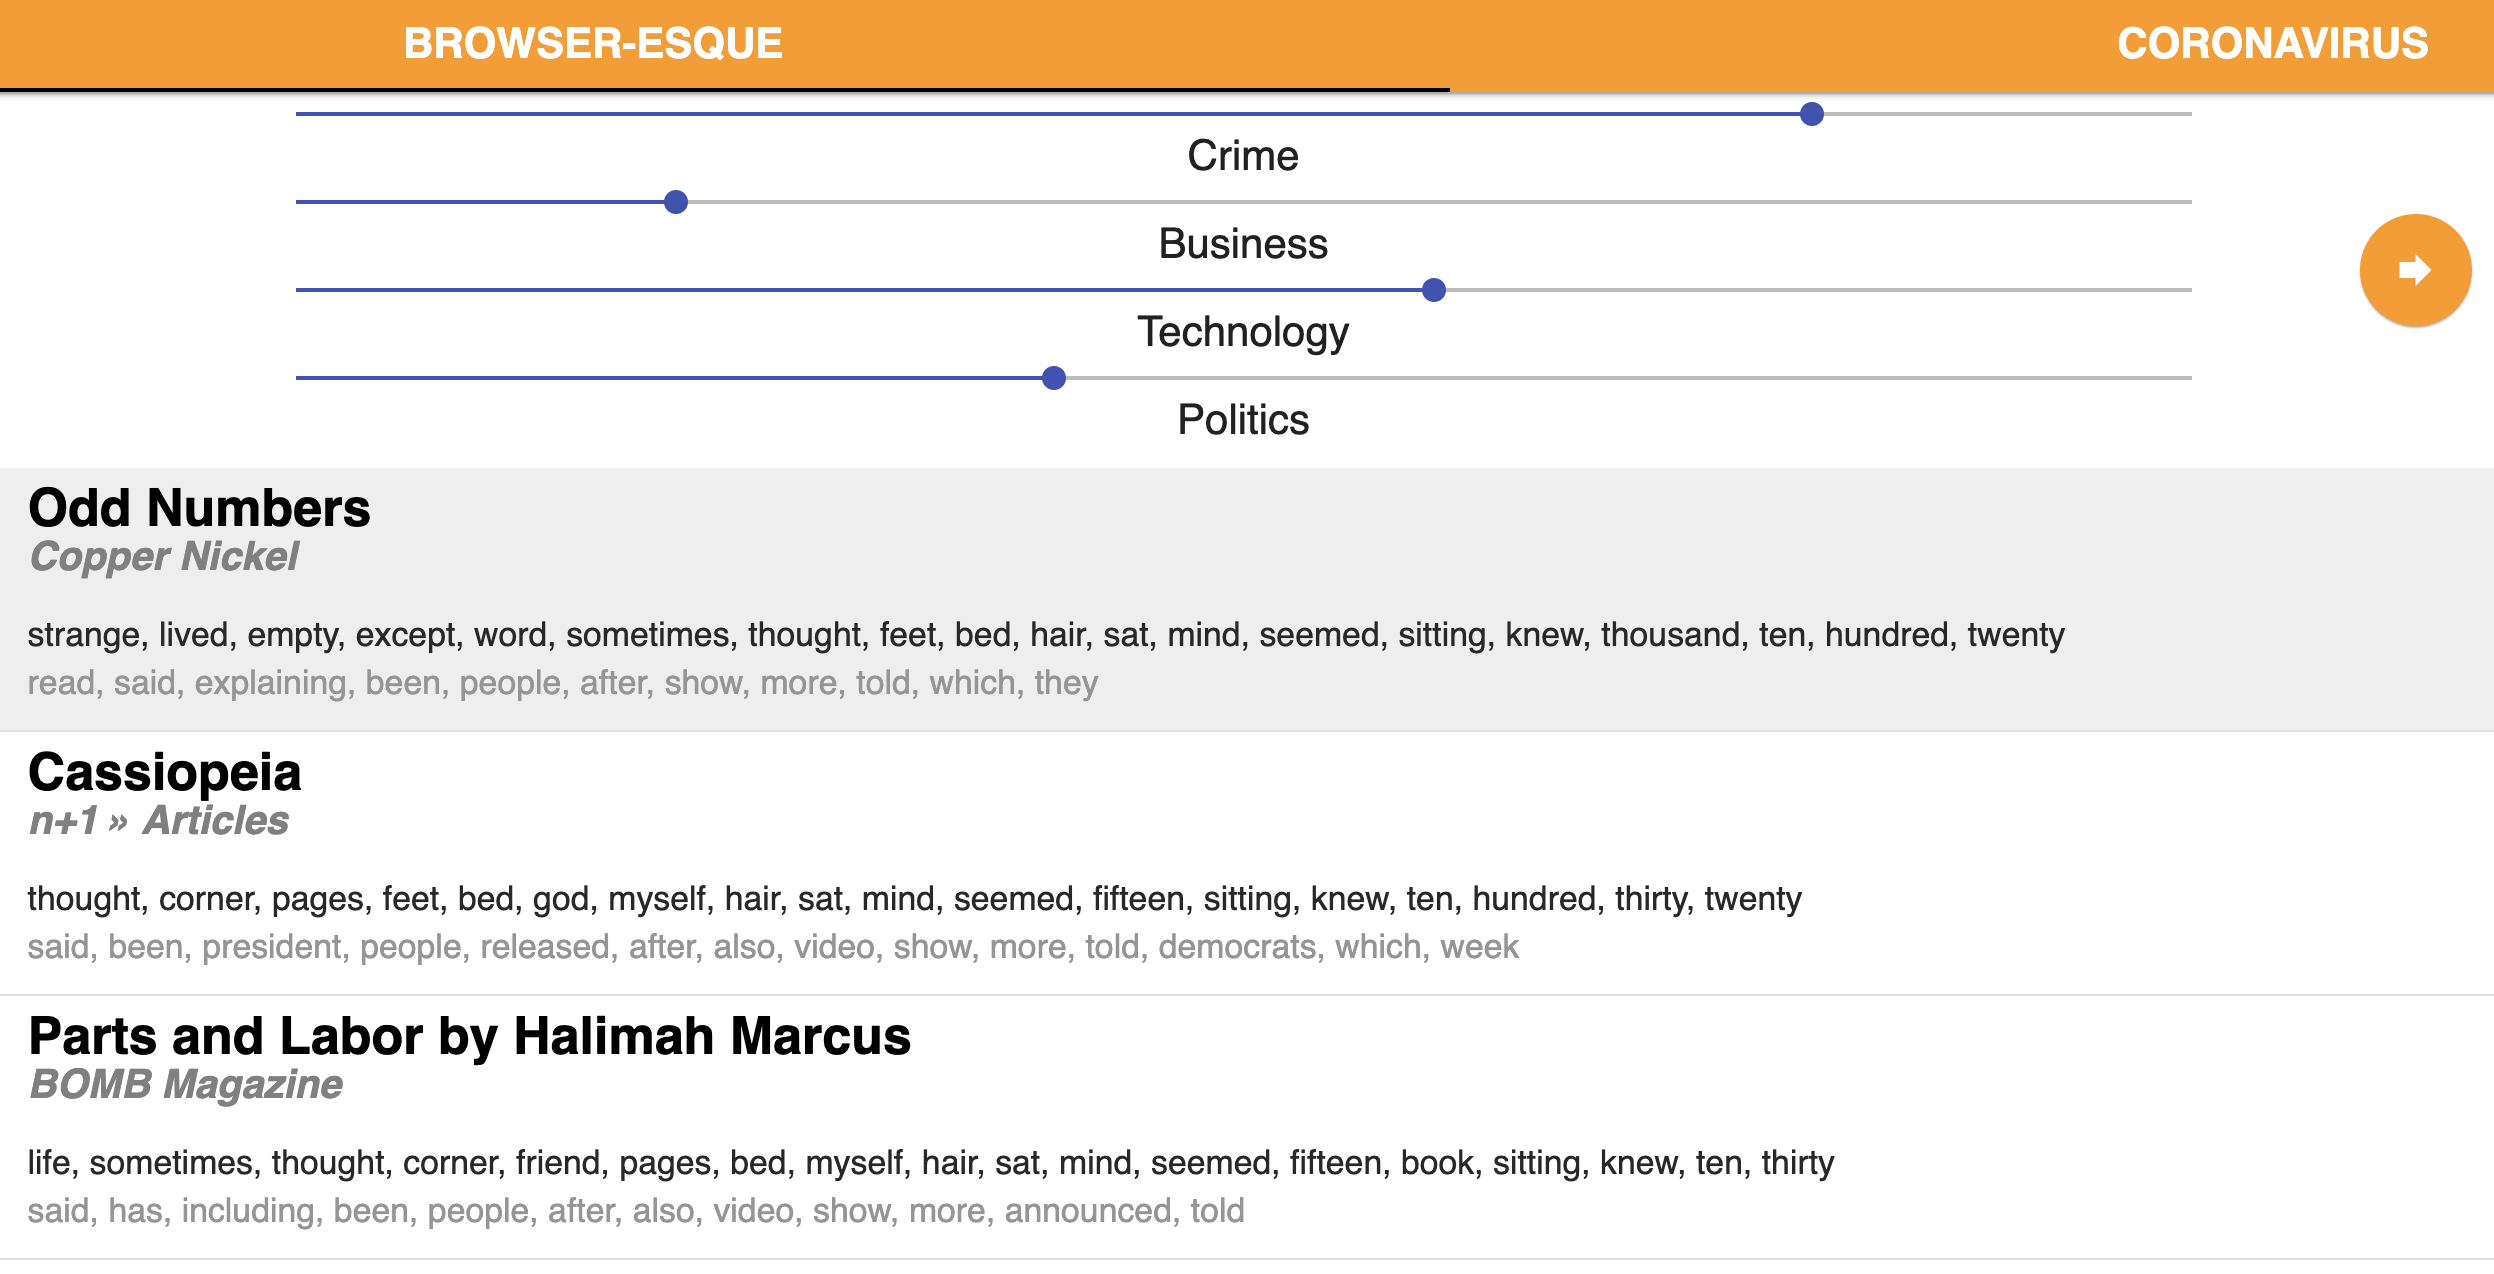
\includegraphics[width=\linewidth]{fig/screen_shots/screen_shot_10.png}
  \caption{Visual interface to \acrlong{rfs} includes topic sliders for setting user preferences as well as most important topic words for each found article}
  \label{fig:screen-shot}
\end{figure}
% !TEX root = recommending-interesting-writing.tex
\section{Recommendation Model}
\acrfull{rfs} is the recommendation model that powers the visual interface; the main part of the pipeline illustrated in \Cref{fig:pipeline}. \gls{rfs} scales to large numbers of articles, and can maximize the evaluation metric of recall~\citep{altosaar2020rankfromsets:,altosaar2020probabilistic}. Recall, or the fraction of true positives returned by a recommendation model, is an appropriate evaluation metric for recommending interesting writing to editors at The Browser. A recommendation model such as \gls{rfs} can be readily backtested with recall as an evaluation metric, as historical data contains positive examples (articles selected by the editors) but rarely contains negative examples (articles seen but not selected by the editors). Further, as our goal is to build an explanation-aware visual interface that can also serve to control recommendations, and \gls{rfs} is fast, interpretable, and simple to integrate into a user interface as we describe later.

\gls{rfs} is a recommendation model defined by a binary classifier. For a user $u$ and item $m$ with attributes $x_m$ (the set of unique words in an article), \gls{rfs} is described by the probability of $y_{um} = 1$ (user $u$ consuming item $m$):
$$p(\yum = 1 \mid u, m) = \sigma\left( f \left (u, x_m\right) \right)\, ,$$
where $\sigma$ is the sigmoid function. To parameterize the binary classifier in \gls{rfs}, we use an inner product architecture:
\begin{equation}
\label{eq:inner-product}
  f\left(u, x_m\right) = \theta_u^\top\left(\frac{1}{|x_m|}\sum_{j\in x_m}
  \beta_j\right)\, .
\end{equation}
In this architecture, the user embedding $\theta_u$ includes a dimension that is fixed to unity. Word embeddings $\beta_j$ (including a bias dimension for every word) and the publication embedding are fit with maximum likelihood estimation, and negative examples are sampled uniformly at random to balance positive examples~\citep{altosaar2020probabilistic}.


% !TEX root = recommending-interesting-writing.tex
\section{Visual Interface}

The visual interface is designed with \gls{rfs} as the backend recommendation model. We describe how the inner product architecture for \gls{rfs} enables a visual interface that is interpretable to provide explanations for why an item is recommended, and enables control so users can filter recommendations to help with decision-making.

\paragraph{Explanation-aware recommendation} The user embedding $\theta_u$ and word embeddings $\beta_j$ in \Cref{eq:inner-product} can be used to interpret a recommendation. The logit for a given document with a set of words $x_m$ is the sum of per-word logits, which are computed as the inner product of the user embedding and word embedding. The per-word contribution of a word in a document to the logit that determines the document's ranking in a list of recommendations is
\begin{equation}
  w_{uj} = \theta_u^\top \beta_j\, .
  \label{eq:word-weight}
\end{equation}
This weight $w_{uj}$ helps explain why a document was recommended, using information about both the user $u$ and the word $j$. In the visual interface, words in a document are first sorted by their contributions to a document's logit $w_{uj}$, and the top words are displayed. Similarly, words that lower a document's ranking are also displayed, to inform a user of which words detract from the recommendation of a document.

\paragraph{Interface for controlling recommendations} In a decision-making task, a user such as an editor for The Browser may wish to filter recommendations according to topics such as crime, technology, or business. The recommendations output by \gls{rfs} can be controlled, by altering the per-word contributions in \Cref{eq:word-weight} according to whether a word is topical. This is accomplished by first calculating words related to a topic word using pre-trained word embeddings from \acrshort{bert}~\citep{devlin2019bert:,wolf2019huggingfaces}. Words related to a topic are defined by a heuristic: the cosine similarity between all words and a topic word such as `business' are computed, and the top $15$ words closest in cosine distance are stored as topical words. Then, a slider in a visual interface is used to increase or decrease the per-word contributions of topical words to a document's logit. Let the user-input slider value be $\alpha$, and the set of topical word indices be $T$. Then the user-controlled version of \Cref{eq:inner-product} becomes
\begin{equation}
\label{eq:inner-product-control}
  f\left(u, x_m\right) = \theta_u^\top\left(\frac{1}{|x_m|}\sum_{j\in x_m}
  (1 - \mbI[j \in T])\beta_j + \mbI[j \in T]\alpha \textrm{sgn}(w_{uj})\beta_j\right)\, .
\end{equation}
The sign function $\textrm{sgn}(~\cdot~)$ is applied to the per-word contribution to a document's logit. This is included since a word might contribute negatively to a document's logit, yet a user may wish to increase the weight of a related topical word.

% !TEX root = recommending-interesting-writing.tex
\section{Evaluation}
\label{sec:experiments}

We conduct an offline empirical study of the performance of \acrlong{rfs} to assess its performance as a recommendation model. Then we qualitatively evaluate the visual interface to study whether the explanation-aware, controllable interface enabled by \gls{rfs} can help make editors at The Browser make better decisions.

\paragraph{Data Collection and Preprocessing.} For positive examples, we use the historical set of articles curated by editors at The Browser. We augment the training data with articles selected by the editors of other curation services, and treat all positively-labeled examples curated by editors as data from a single user due to a paucity of data. We use articles from news websites as examples with negative labels, and collect additional articles with negative labels from websites most-featured by the editors to mimic the editorial process of reading a large swath of articles in a feed and distilling an article list to a select few. For preprocessing the data we use the tokenizer released by \textcite{devlin2019bert:} and discard words not recognized by the tokenizer. This procedure results in a dictionary with $30$k words, and $646$k datapoints with $27$k positive labels.

\paragraph{Metrics} Performance of the recommendation models is assessed with recall, and $15\%$ of the datapoints are held out for the validation and test sets respectively.

\paragraph{Experimental setup: RankFromSets} We cross-validate using the RMSProp optimizer~\parencite{tieleman2012lecture} with a momentum of $0.9$ and grid search over learning rates of $\{10^{-2}, 10^{-3}, 10^{-4}, 10^{-5}\}$, whether or not to initialize from pre-trained \acrshort{bert} embeddings~\parencite{wolf2019huggingfaces}, and embedding sizes of $\{10,25,50, 100, 500, 1000\}$. This model is trained on an NVIDIA Tesla P100 GPU.

\paragraph{Experimental setup: \acrshort{bert}} To fine-tune \acrshort{bert}, we use the AdamW optimizer with a linear learning rate scheduler and warmup steps, with a batch size of $32$ and maximum input length of $512$ as in \textcite{devlin2019bert:} and \textcite{wolf2019huggingfaces}. A grid search is performed over learning rates of $\{2, 3, 4, 5\} \times 10^{-5}$, warmup steps of $\{10^2, 10^3, 10^4\}$, and total training steps of $\{10^2, 10^3, 10^4, 10^5\} \times 5$. The model is trained on an NVIDIA Tesla V100 GPU.

The best-performing model of \gls{rfs} is selected for deployment, and recall is evaluated on the test set, after using early stopping according to validation recall. The results are shown in \Cref{tab:recall}, and \gls{rfs} outperforms \acrshort{bert} by $14\%$. Further, \gls{rfs} achieves better performance ten times faster than \acrshort{bert}, as shown in \Cref{fig:training-recall}. In a test to measure the speed of recommending $10^4$ held-out articles, \gls{rfs} ranked all articles in $120$ ms on a CPU, while \acrshort{bert} took $4$ m $54$ s to rank the articles on an NVIDIA Tesla V100 GPU. This represents a 2000-fold improvement in speed, which is beneficial for the controllable visual interface that requires \Cref{eq:inner-product-control} to be quickly computed in response to user input.

% !TEX root = ../recommending-interesting-writing.tex
\begin{figure}[!tb]
  \centering
  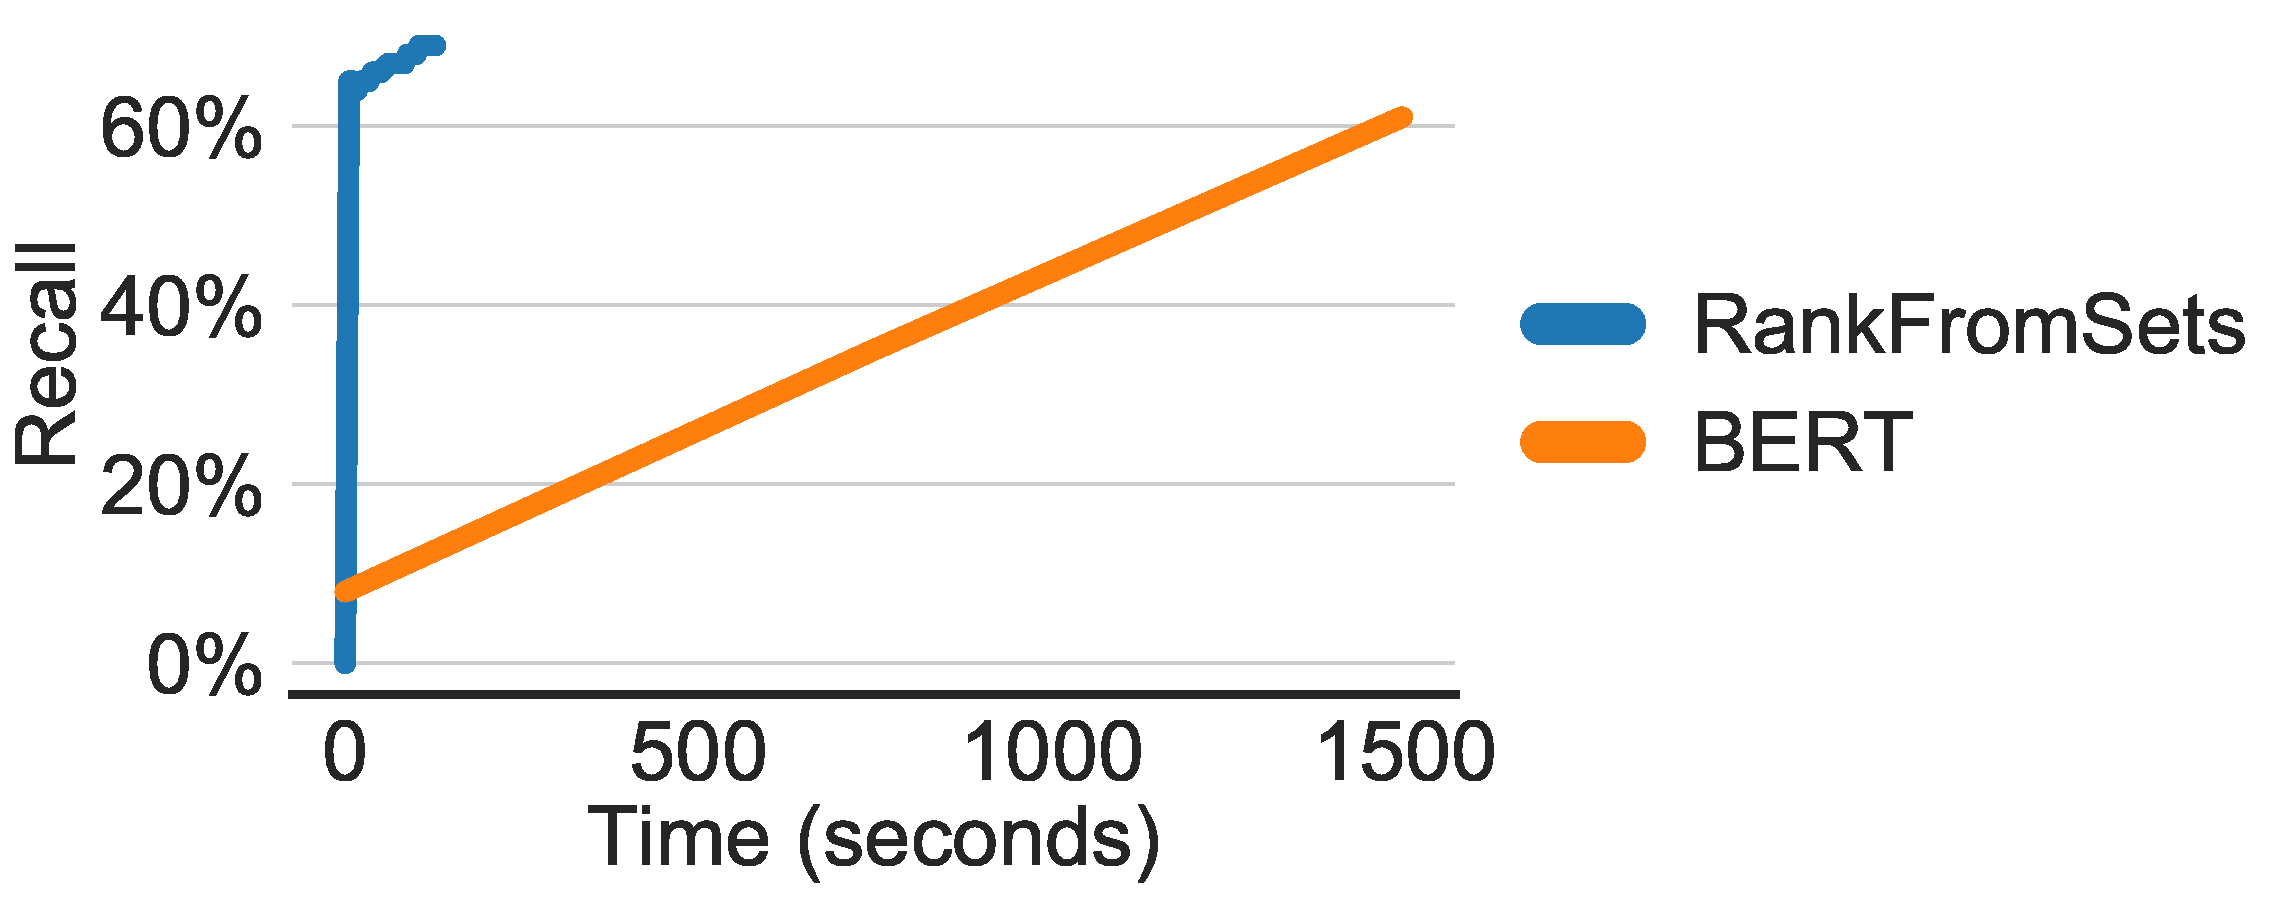
\includegraphics[width=0.95\linewidth]{fig/training-recall}
  \caption{\acrlong{rfs} achieves better performance faster than \acrshort{bert} in terms of validation recall during training.}
  \label{fig:training-recall}
\end{figure}
% !TEX root = ../recommending-interesting-writing.tex
\begin{table}[tb]
\centering
\begin{tabular}{lSS}
\toprule
Recommendation Model & \multicolumn{1}{c}{Recall @ 1000 (\%)}
\\
\midrule
\acrlong{rfs} &  \bfseries 53.1\\
\acrshort{bert} & 46.6 \\
\bottomrule
\end{tabular}
% BERT 466/1000
% rankfromsets 531/1000
% \vspace{1ex}
\caption{\gls{rfs} outperforms \acrshort{bert} in an offline evaluation, on a task of predicting which articles editors at The Browser would feature based on words in the articles.}
\label{tab:recall}
\end{table}

\paragraph{Qualitative Evaluation} In a user study, editors at The Browser provided feedback that they used the visual interface to choose articles, and found this to be an improved workflow. The control over recommendations, and explanation-aware visual interface provided by \gls{rfs} helped elicit bugs in data collection (such as foreign language sources, or fiction writing) and provides an enjoyable user experience.
% !TEX root = recommending-interesting-writing.tex
\section{Deployment}
The visual interface is deployed on Github Pages, with the backend, \gls{rfs}, deployed as a microservice on Amazon Web Services Lambda. \Cref{eq:inner-product-control} is cheap to compute, so the lambda function is a short python script that requires numpy as a dependency, compared to \acrshort{bert} which would require a hosted GPU solution. \gls{rfs} recommends recent articles from the editors' reading list of feeds. As a proof of concept, we include a tab for coronavirus-related articles that users can search through using the sliders and \Cref{eq:inner-product-control}.
% !TEX root = recommending-interesting-writing.tex
\section{Discussion}
\paragraph{Evaluation.} Qualitatively, editors at The Browser preferred the recommendations of our pipeline over their current workflow of a reading list sorted in terms of recency and use the system in production.

\paragraph{Future Work.} Comparing to transformer-based models~\citep{devlin2019bert:} would help clarify how much performance is given up when choosing an efficient model such as \gls{rfs} for recommendations. For explainability beyond top words in an article contributing to a recommendation, it would be interesting to develop methods for enabling editors to search through interpretable latent dimensions. Building quantitative human-in-the-loop evaluation methods into a user interface may also help guide modeling choices. Finally, studying whether the transparency provided by open-source recommendation systems can improve user experience is an open problem.
\section*{Acknowledgments}
The authors are grateful to Christian Bjartli for help with data collection.
% BALANCE COLUMNS
\balance{}

% REFERENCES FORMAT
% References must be the same font size as other body text.
\newcommand{\newblock}{}
%\bibliographystyle{SIGCHI-Reference-Format}
%\bibliography{bib}
\printbibliography
\end{document}

%%% Local Variables:
%%% mode: latex
%%% TeX-master: t
%%% End:
